\section{Review}

\subsection{Polynomial Interpolation}
We have data for a function $f$ aat $x_0, x_1, \dots, x_n$

\subsection{Lagrange Interpolation}
\[
  \sum_{j=0}^n f(x_j) \underbrace{L_j(x)}_{0 \text{ at } x_i \text{ when } i \neq j}
.\]

Reminder: a degree $n$ polynomial interpolant for $n+1$ points is unique. This
means any polynomial interpolation method will give the same polynomial, just in
a different form.

\subsection{Divided Differences}

Divided differences is an easy way to add data points.

Assume we know $f(x)$ at several values for $x$.

% \begin{table}[h]
%   \centering
%   \begin{tabular}{cccc}
%     f_0 & f_1 & f_2 & f_3 \\
%     \hline
%     x_0 & x_1 & x_2 & x_3
%   \end{tabular}
% \end{table}

The $x_i$ points do \uline{not} need to be evenly spaced, or in any particular order.

We choose to represent our degree $n$ interpolating polynomial as follows:

\[
  P_n(x) = a_0 + a_1 (x-x_0) + a_2 (x-x_0) (x-x_1) + \dots + a_n (x-x_0) \dots (x-x_{n-1})
.\]

For every term we add, we interpolate another data point. We choose $a_i$ such
that $P_n(x) = f(x)$ at the points $x_0, x_1, \dots, x_n$.

The coefficients $a_i$ are determined by divided differences

\[
P_n (x_0) = f(x_0)
.\]

\[
  a_0 = f(x_0) = f[x_0]
.\]

Define the zero$^{th}$ divided difference

\[
  f[x_j] = f(x_j)
.\]

\[
a_0 + a_1(x_1-x_0) = f(x_1)
.\]

\[
  f[x_0] + a_1 (x_1-x_0) = f[x_1]
.\]

\[
a_1 = \frac{f[x_1] - f[x_0]}{x_1-x_0}
.\]

Define first divided difference

\[
  f[x_i, x_{i+1}] = f[x_{i+1}, x_i] = \frac{f[x_{i+1}]-f[x_i]}{x_{i+1}-x_i}
.\]

\[
  a_0 = f[x_0]
.\]

\[
  a_1 = f[x_0, x_1]
.\]

\[
  a_2 = f[x_0, x_1, x_2]
.\]

Define the second divided difference

\begin{align*}
  &f[x_i, x_{i+1}, x_{i+2}] \\
  &= \frac{f[x_{i+1}, x_{i+2}] - f[x_i, x_{i+1}]}{x_{i+2}-x_i} \\
\end{align*}

Define the $k^{th}$ divided difference for $x_i, \dots, x_{i+k}$

\begin{align*}
  &f[x_i, x_{i+1}, \dots, x_{i+k}] \\
  &= \frac{f[x_{i+1}, \dots, x_{i+k}] - f[x_i, \dots, x_{i+k-1}]}{x_{i+k}-x_i} 
\end{align*}

\[
  a_k = f[x_0, x_1, \dots, x_k]
.\]

This is Newton's interpolating divided difference formula.


\begin{align*}
  P(x) &= f[x_0] + f_[x_0, x_1] (x-x_0) \\
       &+ f[x_0, x_1, x_2] (x-x_0) (x-x_1) \\
       &+ \dots \\
       &+ f[x_0, x_1, \dots, x_n](x-x_0) \dots (x-x_{n-1})
\end{align*}

To compute an extra datapoint, we only need to compute one more term:

\[
  P_n(x) = P_{n-1}(x) + f[x_0, x_1, \dots, x_n](x-x_0) \dots (x-x_{n-1})
.\]

Note that while using this method, we do NOT need to have our $x_i$ points in
any particular order.

\subsubsection{Example}

\[
  (x_0, \dots, x_4) = (0.3, 1.0, 0.7, 0.6, 1.9)
.\]

Note that our points are not in order, or evenly spaced.

We are going to interpolate 

\[
  f(x) = 2x^3 - x^2 +x - 1
.\]

We can use a table!

Divided differences table:

% \begin{table}[h]
%   \centering
%   \begin{tabular}{c|c|c}
%     \( x_i \) & \( f[x_i] \) & f[x_i, x_{i+1}] \\
%     \hline
%     \( 0.3 \) & \( -0.736 \) & 2.48\\
%     \( 1.0 \) & \( 1.0 \) & 3.68\\
%     \( 0.7 \) & \( -0.104 \) & 2.24\\
%     \( 0.6 \) & \( -0.328 \) & 8.72\\
%     \( 1.9 \) & \( 11.008 \)
%   \end{tabular}
% \end{table}

\begin{center}
    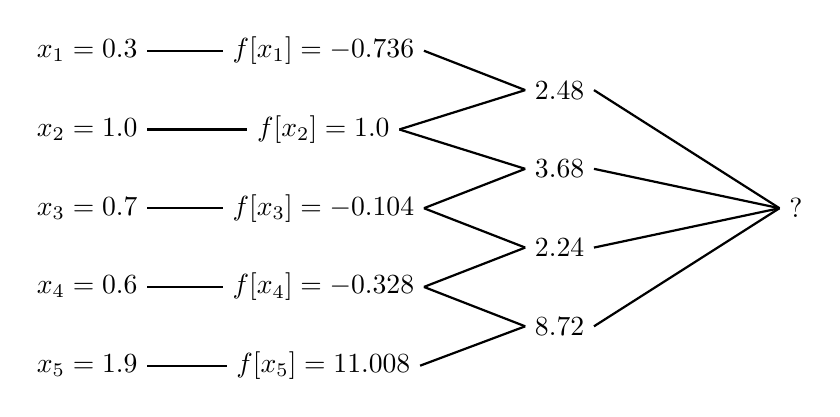
\begin{tikzpicture}
        % Nodes (x_i values)
        \node (X1) at (0, 4) {\( x_1 = 0.3 \)};
        \node (X2) at (0, 3) {\( x_2 = 1.0 \)};
        \node (X3) at (0, 2) {\( x_3 = 0.7 \)};
        \node (X4) at (0, 1) {\( x_4 = 0.6 \)};
        \node (X5) at (0, 0) {\( x_5 = 1.9 \)};

        % Nodes (f[x_i] values)
        \node (F1) at (3, 4) {\( f[x_1] = -0.736 \)};
        \node (F2) at (3, 3) {\( f[x_2] = 1.0 \)};
        \node (F3) at (3, 2) {\( f[x_3] = -0.104 \)};
        \node (F4) at (3, 1) {\( f[x_4] = -0.328 \)};
        \node (F5) at (3, 0) {\( f[x_5] = 11.008 \)};

        % Nodes (Third Column)
        \node (C1) at (6, 3.5) {\( 2.48 \)};
        \node (C2) at (6, 2.5) {\( 3.68 \)};
        \node (C3) at (6, 1.5) {\( 2.24 \)};
        \node (C4) at (6, 0.5) {\( 8.72 \)};

        % Final Result Node
        \node (Final) at (9, 2) {\( ? \)};

        % Connecting Lines (Tree Structure)
        \draw[thick] (X1.east) -- (F1.west);
        \draw[thick] (X2.east) -- (F2.west);
        \draw[thick] (X3.east) -- (F3.west);
        \draw[thick] (X4.east) -- (F4.west);
        \draw[thick] (X5.east) -- (F5.west);

        \draw[thick] (F1.east) -- (C1.west);
        \draw[thick] (F2.east) -- (C1.west);
        \draw[thick] (F3.east) -- (C2.west);
        \draw[thick] (F4.east) -- (C3.west);
        \draw[thick] (F5.east) -- (C4.west);

        \draw[thick] (F2.east) -- (C2.west);
        \draw[thick] (F3.east) -- (C3.west);
        \draw[thick] (F4.east) -- (C4.west);


        \draw[thick] (C1.east) -- (Final.west);
        \draw[thick] (C2.east) -- (Final.west);
        \draw[thick] (C3.east) -- (Final.west);
        \draw[thick] (C4.east) -- (Final.west);

    \end{tikzpicture}
\end{center}

The first entry in each column gives the coefficients

\begin{align*}
    P_4(x) &= -0.736 \\
           &\quad + 2.48(x-0.3) \\
           &\quad + 3(x-0.3)(x-1.0) \\
           &\quad + 2(x-0.3)(x-1.0)(x-0.7) \\
           &\quad + 0(x-0.3)(x-1.0)(x-0.7)(x-0.6) \\
           &\quad + 0(x-0.3)(x-1.0)(x-0.7)(x-0.6)(x-1.9).
\end{align*}

\section{KEY TAKEAWAY}

Basically, using the table, we can get all the constants we need to compute the
next datapoint by just looking back and grabbing the appropriate column.

\section{Midterm Review}

Find the rate of convergence as $h\to 0$:

\[
  \lim_{h \to 0} (e^h + e^{-h}) = 2
.\]

1. expand $e^h + e^{-h} - 2$ using taylor series

\[
  e^h = 1+h + \frac{h^2}{2!} + \frac{h^3}{3!} + O(h^4)
.\]


\begin{align*}
  e^h + e^{-h} -2 &= \left(1+h + \frac{h^2}{2!} + \frac{h^3}{3!} + O(h^4) \right ) \\
                  &\quad + \left ( 1-h+\frac{h^2}{2!}-\frac{h^3}{3!}+O(h^4) \right ) \\
                  &-2 \\
                  &= h^2 + O(h^3) = O(h^2)
\end{align*}

For midterm, know:
\begin{itemize}
  \item common taylor series 
    % ($e^x, \sin(x), \cos(x), \ln(1+x), (1+x)^{-p}$) 
  \item Partial Pivoting w/ or w/0 scaling
\end{itemize}

\subsection{Another Problem}

Consider

\begin{align*}
  x_1 + 30x_2 &= 50 \\
  5x_1 - 10x_2 &=  3
\end{align*}

Use Gaussian Elimination w/ scaled partial pivoting to take the system to upper
triangular form.

$\displaystyle \frac{1}{30} < \frac{5}{10} \implies$ we need to exchange rows

\begin{align*}
  5x_1 - 10x_2 &=  3 \\
   x_1 + 30x_2 &= 50 \\
  \hline
  5x_1 - 10x_2 &=  3 \\
  32x_2 = 50 - \frac{3}{5}
\end{align*}

